% +------------------------------------------------------------------------+
% | Reference manual page: Subdivision_method_3.tex
% +------------------------------------------------------------------------+
% | 03/01/2005   Le-Jeng Andy Shiue
% | Package: Subdivision_surface_3
% | 
\RCSdef{\RCSSubdivisionRev}{$Id$}
\RCSdefDate{\RCSSubdivisionDate}{$Date$}
% +------------------------------------------------------------------------+

\ccRefPageBegin

%%RefPage: end of header, begin of main body
% +------------------------------------------------------------------------+


% +------------------------------------------------------------------------+
% +------------------------------------------------------------------------+
\begin{ccRefClass}{CatmullClark_mask_3<Polyhedron_3>}

\ccDefinition

A stencil determines a source neighborhood 
whose points contribute to the position of a refined point.
The geometry mask of a stencil specifies
the computation on the nodes of the stencil.
\ccClassTemplateName\ implements the geometry masks of 
Catmull-Clark subdivision on a \ccc{Polyhedron_3<Cartesian>}.

\ccInclude{CGAL/Subdivision_mask_3.h}

\ccParameters

The full template declaration of \ccClassTemplateName\ states one
template parameter:

\begin{tabbing}
\ccc{template <} \=\ccc{class Polyhedron_3>} \ccc{class CatmullClark_mask_3;}
\end{tabbing}
   
The only parameter requires a \ccc{Polyhedron_3} as the argument. The
\ccc{Polyhedron_3} should be specialized with the \ccc{Cartesian}
kernel, which defines the \ccc{Point_3} for the vertices.

\ccCreation
\ccCreationVariable{CC}

\ccConstructor{CatmullClark_mask_3<Polyhedron_3>();}{default constructor.}

% +-----------------------------------+
\ccHeading{Stencil functions}
%\ccThree{void}{facet_node(Facet_handle f, Point& pt);}{}
\ccThree{void}{CC.nn}{}
\ccThreeToTwo

\ccMethod{
void facet_node(Facet_handle f, Point_3& pt);
}{
computes the Catmull-Clark facet-point \ccc{pt} of the facet \ccc{f}.
}

\ccMethod{
void edge_node(Edge_handle e, Point_3& pt);
}{
computes the Catmull-Clark edge-point \ccc{pt} of the edge \ccc{e}.
}

\ccMethod{
void vertex_node(Vertex_handle v, Point_3& pt);
}{
computes the Catmull-Clark vertex-point \ccc{pt} of the vertex \ccc{v}.
}

\ccMethod{
void border_node(Halfedge_handle e, Point_3& ept, Point_3& vpt);
}{
computes the Catmull-Clark edge-point \ccc{ept} and the 
Catmull-Clark vertex-point \ccc{vpt} of the border edge \ccc{e}.
}
\begin{ccTexOnly}
  \begin{center}
    \parbox{0.75\textwidth}{%
      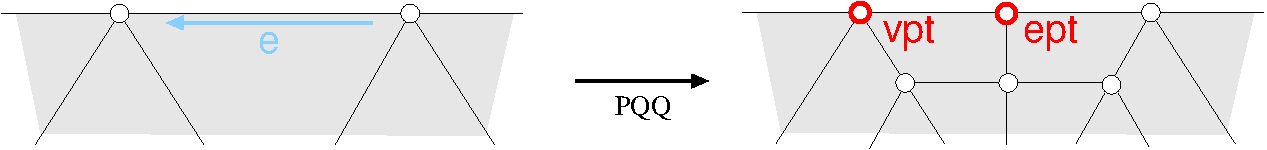
\includegraphics[width=0.75\textwidth]{Subdivision_method_3_ref/FIG/CCBorderMask}%
    }
  \end{center}
\end{ccTexOnly}

\begin{ccHtmlOnly}
    <CENTER>
      <img src="FIG/CCBorderMask.png" alt="PQQ stencil of border nodes"></A><P>
    </CENTER>
\end{ccHtmlOnly}

\ccSeeAlso

\ccRefIdfierPage{CGAL::Subdivision_method_3}\\
%%\ccRefIdfierPage{CGAL::PQQ_stencil_3<Polyhedron_3>}\\
%%\ccRefIdfierPage{CGAL::Linear_mask_3<Polyhedron_3>}\\

\end{ccRefClass}

% +------------------------------------------------------------------------+
%%RefPage: end of main body, begin of footer
\ccRefPageEnd
% EOF
% +------------------------------------------------------------------------+


% +------------------------------------------------------------------------+
% +------------------------------------------------------------------------+
\begin{ccRefClass}{Loop_mask_3<Polyhedron_3>}

\ccDefinition

A stencil determines a source neighborhood 
whose points contribute to the position of a refined point.
The geometry mask of a stencil specifies
the computation on the nodes of the stencil.
\ccClassTemplateName\ implements the geometry masks of 
Loop subdivision on a triangulated \ccc{Polyhedron_3<Cartesian>}.

\ccInclude{CGAL/Subdivision_mask_3.h}

\ccParameters

The full template declaration of \ccClassTemplateName\ states one
template parameter:

\begin{tabbing}
\ccc{template <} \=\ccc{class Polyhedron_3>} \ccc{class Loop_mask_3;}
\end{tabbing}
   
The only parameter requires a \ccc{Polyhedron_3} as the argument. The
\ccc{Polyhedron_3} should be specialized with the \ccc{Cartesian}
kernel, which defines the \ccc{Point_3} for the vertices.

\ccCreation
\ccCreationVariable{L}

\ccConstructor{Loop_mask_3<Polyhedron_3>();}{default constructor.}

% +-----------------------------------+
\ccHeading{Stencil functions}
%\ccThree{void}{edge_node(Edge_handle e, Point& pt);}{}
\ccThree{void}{L.nn}{}
\ccThreeToTwo

\ccMethod{
void edge_node(Edge_handle e, Point_3& pt);
}{
computes the Loop edge-point \ccc{pt} of the edge \ccc{e}.
}

\ccMethod{
void vertex_node(Vertex_handle v, Point_3& pt);
}{
computes the Loop vertex-point \ccc{pt} of the vertex \ccc{v}.
}

\ccMethod{
void border_node(Halfedge_handle e, Point_3& ept, Point_3& vpt);
}{
computes the Loop edge-point \ccc{ept} and the 
Loop vertex-point \ccc{vpt} of the border edge \ccc{e}.
}

\begin{ccTexOnly}
  \begin{center}
    \parbox{0.75\textwidth}{%
      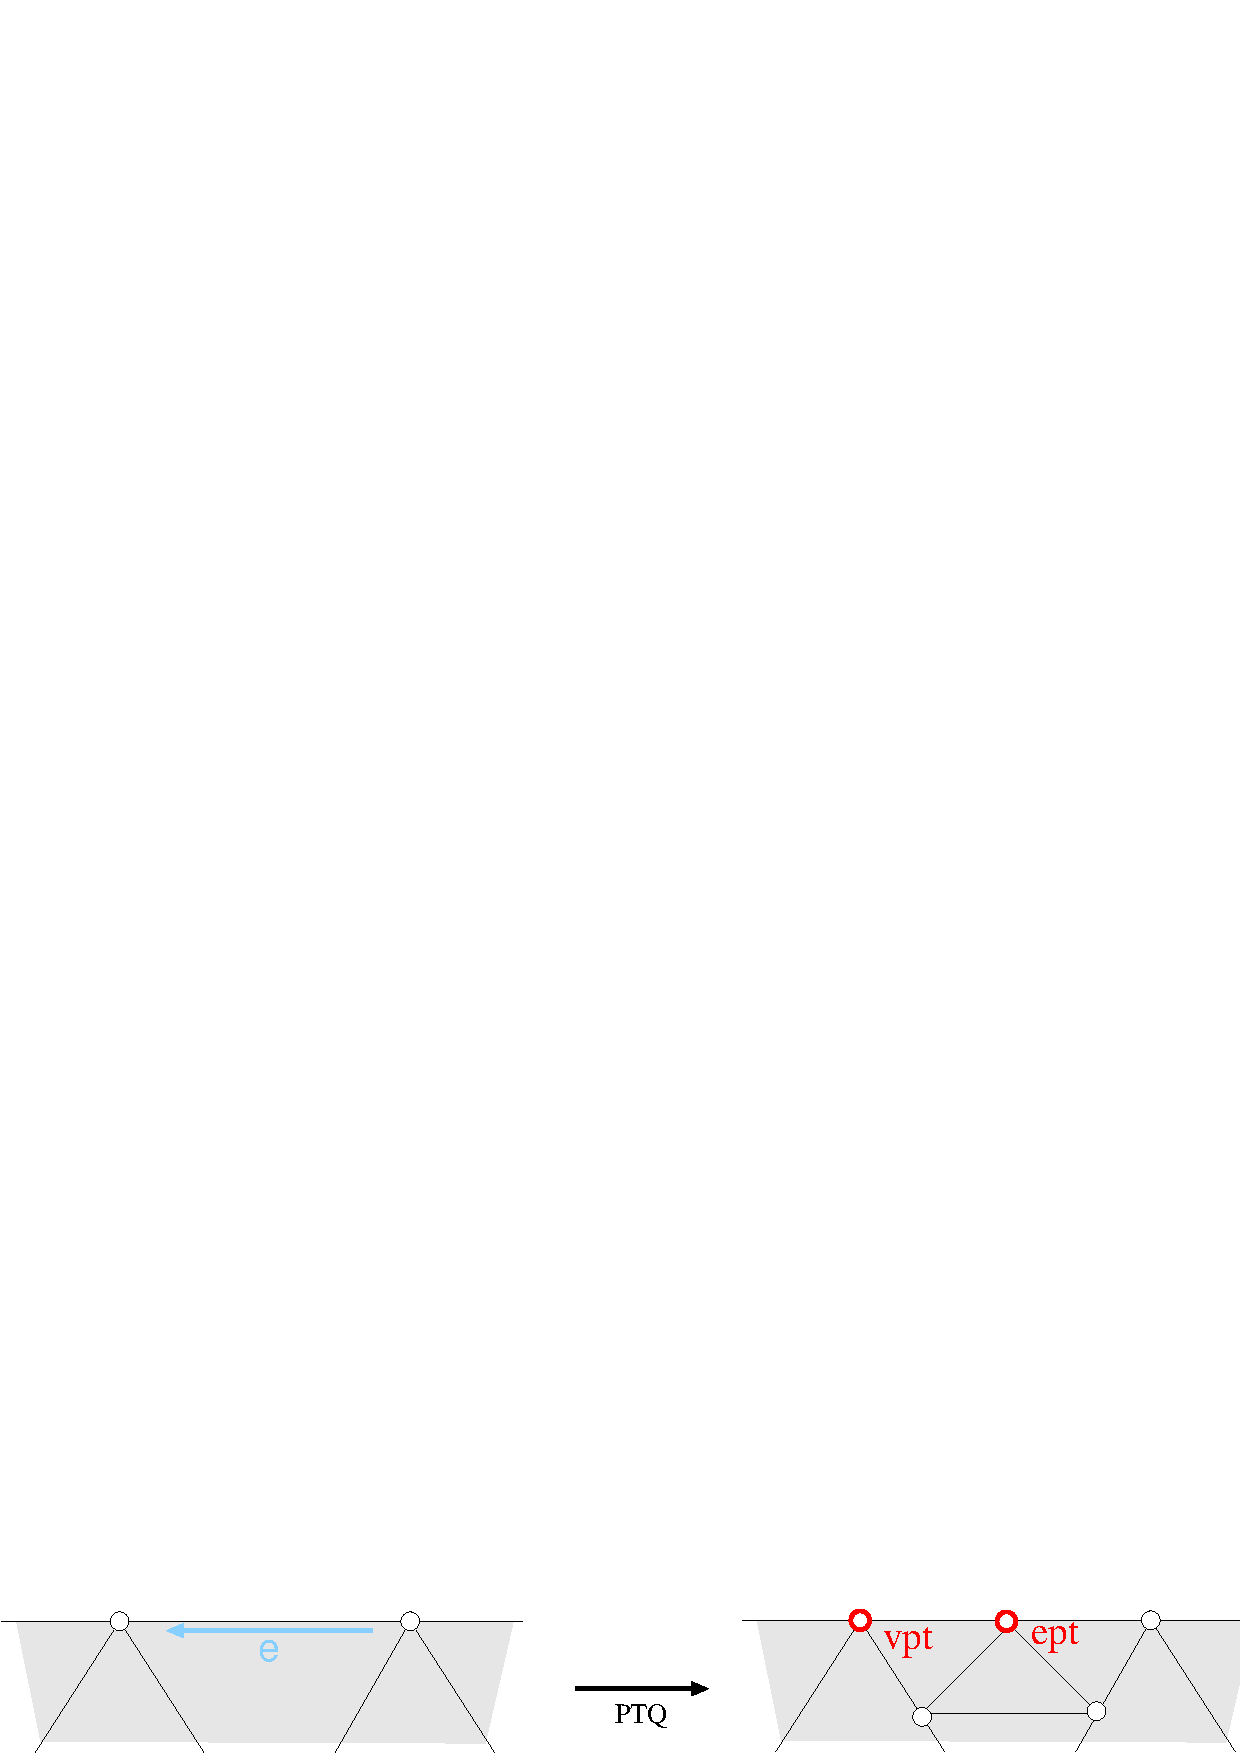
\includegraphics[width=0.75\textwidth]{Subdivision_method_3_ref/FIG/LoopBorderMask}%
    }
  \end{center}
\end{ccTexOnly}

\begin{ccHtmlOnly}
    <CENTER>
      <img src="FIG/LoopBorderMask.png" alt="PTQ stencil of border nodes"></A><P>
    </CENTER>
\end{ccHtmlOnly}

\ccSeeAlso

\ccRefIdfierPage{CGAL::Subdivision_method_3}\\
%%\ccRefIdfierPage{CGAL::PQQ_stencil_3<Poly>}\\

\end{ccRefClass}

% +------------------------------------------------------------------------+
%%RefPage: end of main body, begin of footer
\ccRefPageEnd
% EOF
% +------------------------------------------------------------------------+


% +------------------------------------------------------------------------+
% +------------------------------------------------------------------------+
\begin{ccRefClass}{DooSabin_mask_3<Polyhedron_3>}

\ccDefinition

A stencil determines a source neighborhood 
whose points contribute to the position of a refined point.
The geometry mask of a stencil specifies
the computation on the nodes of the stencil.
\ccClassTemplateName\ implements the geometry masks of 
Doo-Sabin subdivision on a \ccc{Polyhedron_3<Cartesian>}.

\ccInclude{CGAL/Subdivision_mask_3.h}

\ccParameters

The full template declaration of \ccClassTemplateName\ states one
template parameter:

\begin{tabbing}
\ccc{template <} \=\ccc{class Polyhedron_3>} \ccc{class DooSabin_mask_3;}
\end{tabbing}
   
The only parameter requires a \ccc{Polyhedron_3} as the argument. The
\ccc{Polyhedron_3} should be specialized with the \ccc{Cartesian}
kernel, which defines the \ccc{Point_3} for the vertices.

\ccCreation
\ccCreationVariable{DS}

\ccConstructor{DooSabin_mask_3<Polyhedron_3>();}{default constructor.}

% +-----------------------------------+
\ccHeading{Stencil functions}
%\ccThree{void}{corner_node(Halfedge_handle he, Point& pt);}{}
\ccThree{void}{DS.nn}{}
\ccThreeToTwo

\ccMethod{
void corner_node(Halfedge_handle he, Point_3& pt);
}{
computes the Doo-Sabin point \ccc{pt} of the vertex pointed
by the halfedge \ccc{he}.
}

\begin{ccTexOnly}
  \begin{center}
    \parbox{0.55\textwidth}{%
      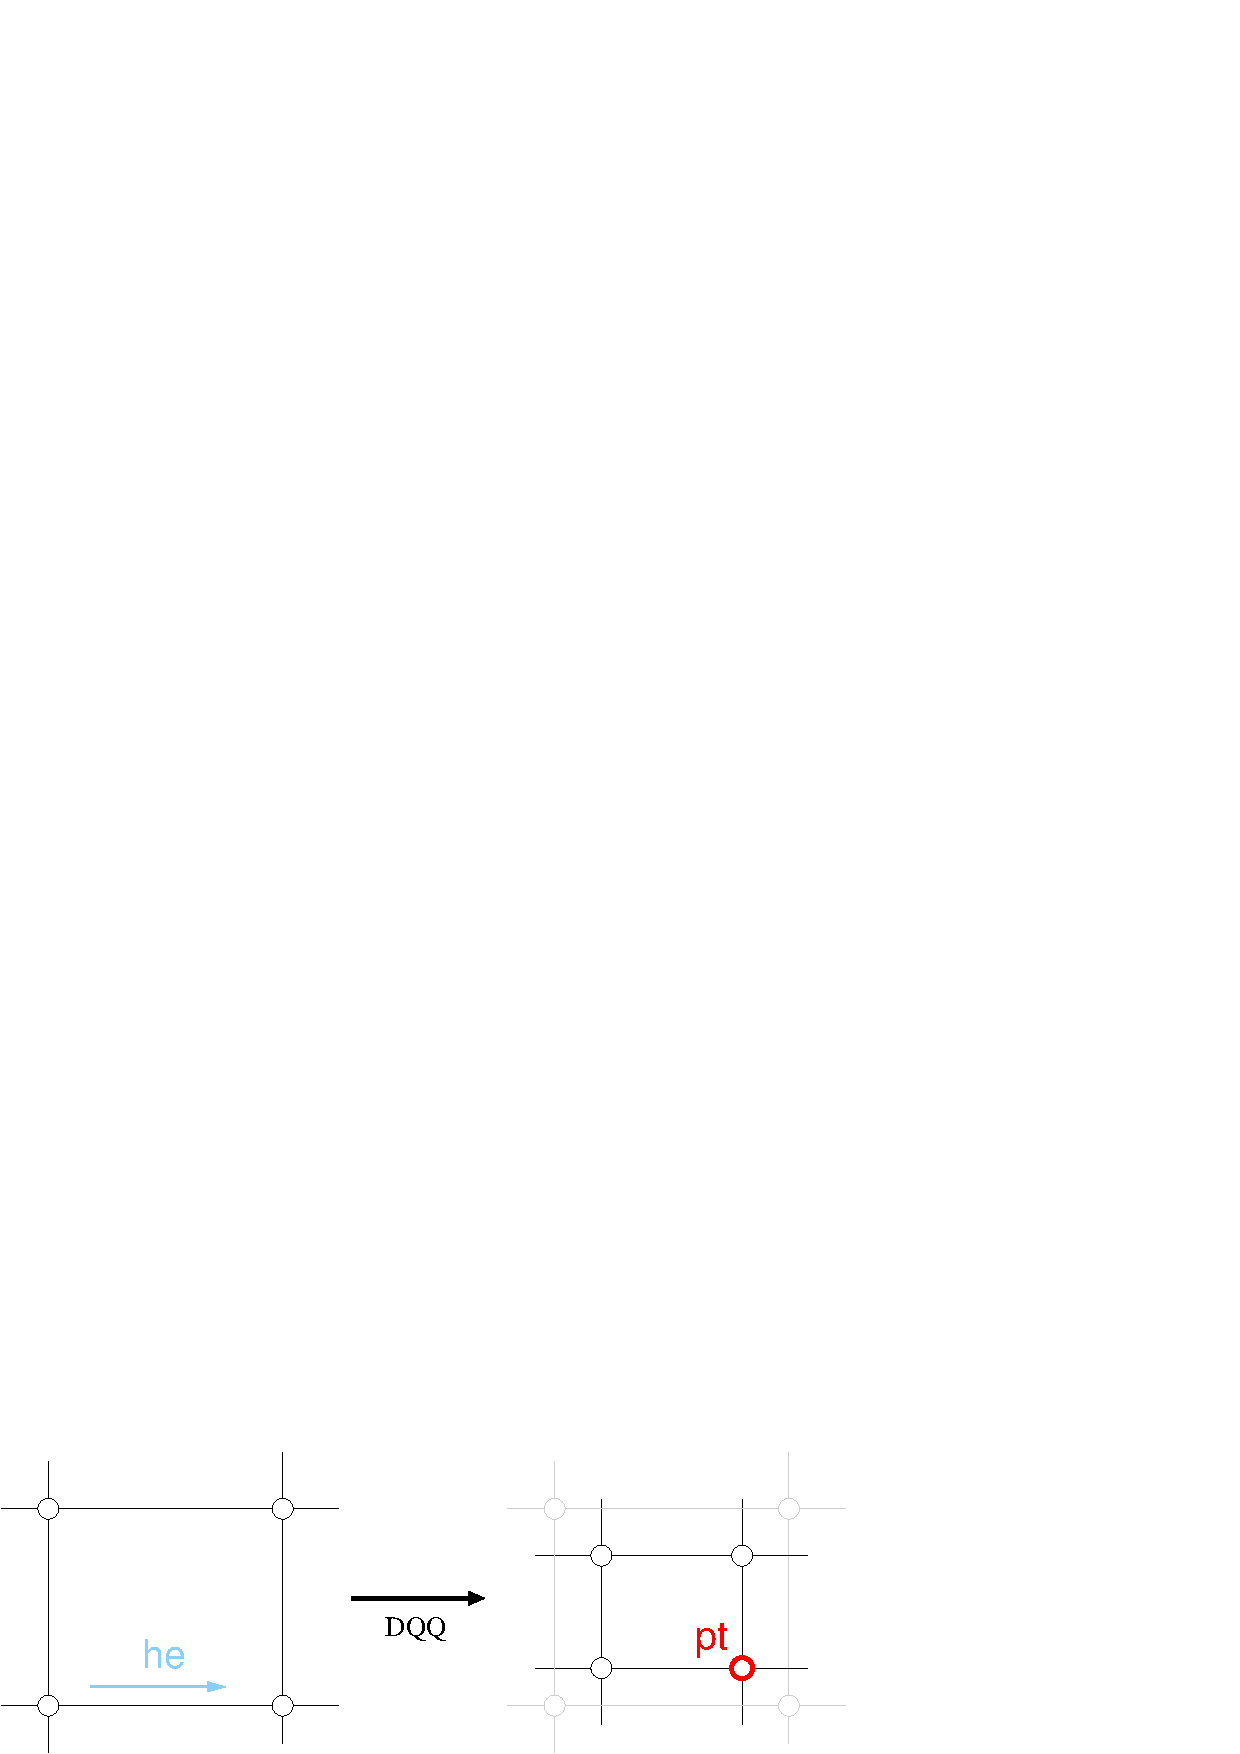
\includegraphics[width=0.55\textwidth]{Subdivision_method_3_ref/FIG/DSCornerMask}%
    }
  \end{center}
\end{ccTexOnly}

\begin{ccHtmlOnly}
    <CENTER>
      <img src="FIG/DSCornerMask.png" alt="DQQ corner stencil"></A><P>
    </CENTER>
\end{ccHtmlOnly}

\ccSeeAlso

\ccRefIdfierPage{CGAL::Subdivision_method_3}\\
%%\ccRefIdfierPage{CGAL::DQQ_stencil_3<Poly>}\\

\end{ccRefClass}

% +------------------------------------------------------------------------+
%%RefPage: end of main body, begin of footer
\ccRefPageEnd
% EOF
% +------------------------------------------------------------------------+


% +------------------------------------------------------------------------+
% +------------------------------------------------------------------------+
\begin{ccRefClass}{Sqrt3_mask_3<Polyhedron_3>}

\ccDefinition

A stencil determines a source neighborhood 
whose points contribute to the position of a refined point.
The geometry mask of a stencil specifies
the computation on the nodes of the stencil.
\ccClassTemplateName\ implements the geometry masks of 
$\sqrt{3}$ subdivision on a triangulated 
\ccc{Polyhedron_3<Cartesian>}.

\ccInclude{CGAL/Subdivision_mask_3.h}

\ccParameters

The full template declaration of \ccClassTemplateName\ states one
template parameter:

\begin{tabbing}
\ccc{template <} \=\ccc{class Polyhedron_3>} \ccc{class Sqrt3_mask_3;}
\end{tabbing}
   
The only parameter requires a \ccc{Polyhedron_3} as the argument. The
\ccc{Polyhedron_3} should be specialized with the \ccc{Cartesian}
kernel, which defines the \ccc{Point_3} for the vertices.

\ccCreation
\ccCreationVariable{S}

\ccConstructor{Sqrt3_mask_3<Polyhedron_3>();}{default constructor.}

% +-----------------------------------+
\ccHeading{Stencil functions}
%\ccThree{void}{facet_node(Facet_handle f, Point& pt);}{}
\ccThree{void}{S.nn}{}
\ccThreeToTwo

\ccMethod{
void facet_node(Facet_handle f, Point_3& pt);
}{
computes the $\sqrt{3}$ facet-point \ccc{pt} of the facet \ccc{f}.
}

\ccMethod{
void vertex_node(Vertex_handle v, Point& pt);
}{
computes the $\sqrt{3}$ vertex-point \ccc{pt} of the vertex \ccc{v}.
}

\ccSeeAlso

\ccRefIdfierPage{CGAL::Subdivision_method_3}\\
%\ccRefIdfierPage{CGAL::PQQ_stencil_3<Poly>}\\
%\ccRefIdfierPage{CGAL::Linear_mask_3<Poly>}\\

\end{ccRefClass}

% +------------------------------------------------------------------------+
%%RefPage: end of main body, begin of footer
\ccRefPageEnd
% EOF
% +------------------------------------------------------------------------+

